\section{SUSIJUSIŲ DARBŲ APŽVALGA}
\label{darbu_apzvalga}

Šiame skyriuje aprašysiu teoriją reikalingą bakalauriniame darbe atliekamam tyrimui: mašininis mokymasis, SVM klasifikatorius, random forest, dimensijų atrinkimo stabilumas.

\subsection{Mokymasis su mokytoju ir mokymasis be mokytojo}

Mašininis mokymasis yra dirbtinio intelekto šaka, kuri siekia įgalinti kompiuterius tobulinti savo elgseną (mokytis) empirinių duomenų atžvilgiu \cite{duda2001pattern}. Pagal tai, kokie yra turimi empiriniai duomenys, mašininis mokymasis yra skirstomas į mokymąsi su mokytoju (angl. \textit{supervised learning}) ir mokymąsi be mokytojo (angl. \textit{unsupervised learning}). Šiame poskyryje aptarsiu, kas yra mokymasis su mokytoju ir mokymasis be mokytojo bei kuo jie skiriasi.

\subsubsection{Mokymasis su mokytoju}

Žmonės mokosi iš patirties, tačiau, skirtingai nei žmonės, kompiuteris patirties neturi, todėl kompiuteris turi mokytis iš patyrimą apibūdinančių duomenų -- mokymosi duomenų. Mašininio mokymosi tikslas yra sukonstruoti funkciją, kuri galėtų būti naudojama nuspėti patyrimą apibūdinančių charakteristikų reikšmes pagal patyrimą apibūdinančius duomenis. Mokymesi su mokytoju, mokytoją reikia suprasti kaip išankstinį mokymosi duomenų spėjamų charakteristikų žinojimą. Kitaip tariant, mokymesi su mokytoju yra sprendžiamas uždavinys, kuriam atsakymą galime pasitikrinti. Pagal tai, kokias charakteristikas bandome nuspėti mokymasis su mokytoju yra skirstomas į dvi rūšis:
\begin{enumerate}
  \item Klasifikavimas (angl. classification) -- pagal mokymosi duomenų nepriklausomus kintamuosius bandoma nuspėti kokybinius (kategorinėd reikšmės) priklausomus kintamuosius.
  \item Regresinė analizė (angl. regression) -- pagal mokymosi duomenų nepriklausomus kintamuosius bandoma nuspėti kiekybinius (tolydinėd reikšmės) priklausomus kintamuosius.
\end{enumerate} 

%% JG: Pateik vizualų klasifikavimo pavyzdį iliustruojanti visus 3 etapus.
%% DJ: Vizualų, ta prasme su paveiksliukais ar ir tas pavyzdys su paštu pakankamai vaizdingas?
%% JG: Reikia kitaip struktūrizuoti šitą skyrių: 
% +Pradžioj pasakyk, kad yra klasifikavimas ir regresija ir po
%  sakinįÂ kiekvienam.
% +Tada aptark klasifikavimą ir pateik pavyzdį. 
% +Tada pateik regresijos pavyzdį.
% +Tada parašyk, kad šiame darbe studijuojama klasifikavimo problema.

\paragraph{Klasifikavimas}

Mašininiame mokymesi klasifikavimu yra vadinama problema, kai pagal mokymosi duomenis reikia nustatyti, kuriai klasei (grupei) priklauso objektas. Klasifikavimo procesas pavaizduotas ~\ref{fig:classification_process} pav. pavaizduota srautų diagrama. Dirbant su biomedicininiais duomenimis tipinė užduotis yra pagal mėginį (pacientą) apibūdinančius matus (patirtį) sukonstruoti klasifikatorių (funkciją), kuris bandys nuspėti, kuriai pacientų grupei -- sergančiųjų ar sveikųjų -- priklauso tiriamasis pacientas.
\begin{figure}
 \centering
 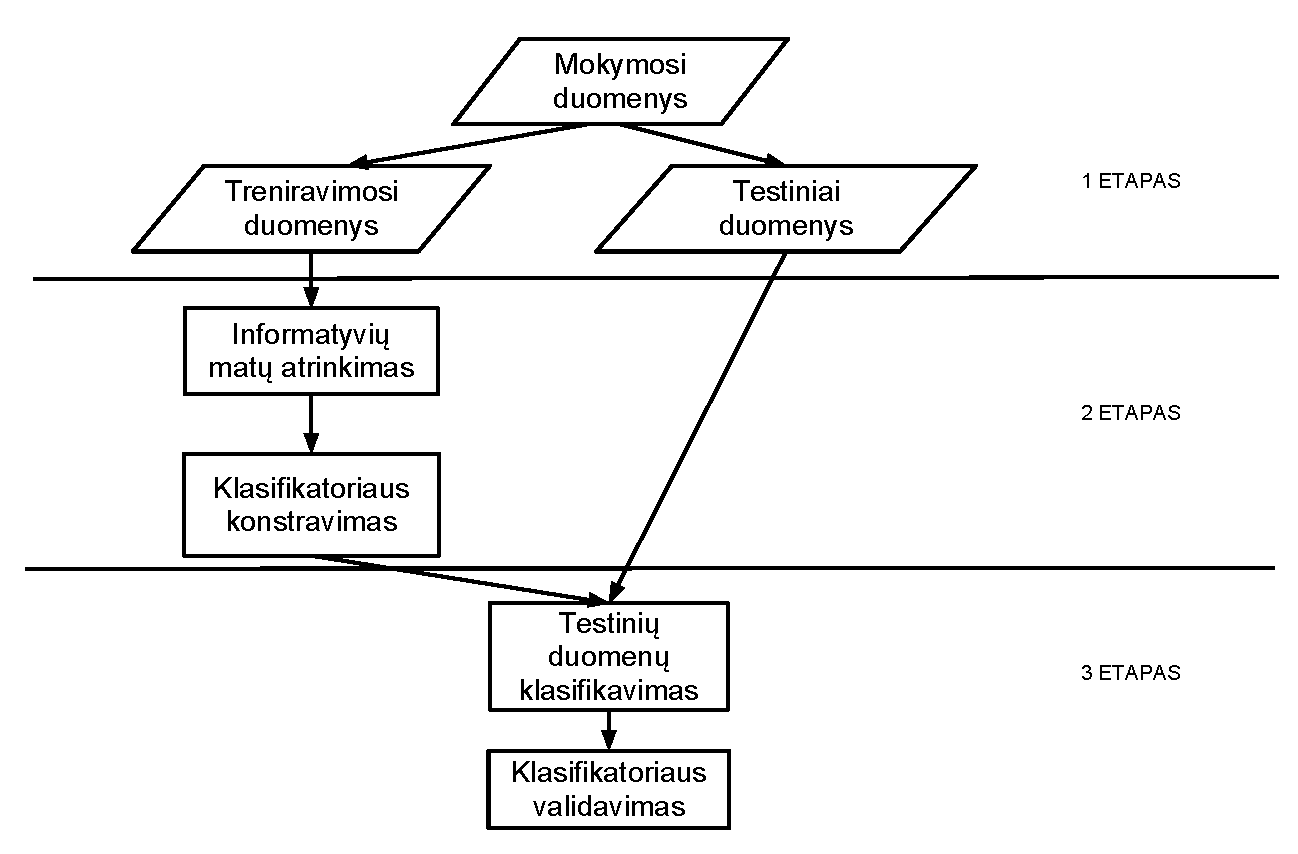
\includegraphics[width=\textwidth]{images/classification_process.pdf}
 \caption{Klasifikavimo srautų diagrama su paaiškinimais.}
 \label{fig:classification_process}
\end{figure}

\paragraph{Regresinė analizė}

Mašininiame mokymesi regresine analize yra vadinama problema, kai pagal patirtį apibūdinančius duomenis reikia nustatyti kiekybines duomenų charakteristikas. Regresinė analizė naudoja standartinius statistinius metodus, tokius kaip mažiausių kvadratų metodas (angl. \textit{least squares}). Regresinė analizė dažniausiai naudojama įvertinti (ang. \textit{forecast}) ateities duomenų vertes bei interpoliacijai -- funkcijos tikėtinos reikšmės tarp keletos taškų įvertinimui. 

Dirbant su biomedicininiais duomenimis regresinė analizė gali būti taikoma bandant nuspėti mėginių trūkstamus matus apibūdinančias reikšmes -- interpoliuoti. Tačiau regresinė analizė dirbant su biomedicininiais duomenimis yra naudojama rečiau negu klasifikavimas, todėl toliau šiame darbe bus nagrinėjama klasifikavimo problema.

%% DJ: Juozai, gal turi gražų pavyzdį, kur pritaikoma regresinė analizė dirbant su biomedicininiais duomenimis?

\subsubsection{Mokymasis be mokytojo}

Mašininio mokymosi kontekste dažnai sutinkamas uždavinys yra į prasmingas grupes (klasterius) sugrupuoti turimus duomenis, apie kuriuos nieko nėra žinoma. Kitaip tariant, reikia išspręsti duomenų grupavimo uždavinį, kuriam neturima iš anksto teisingo atsakymo. Mokymasis be mokytojo tai toks mokymasis, kai teisingas mokymosi duomenų grupavimas iš anksto nėra žinomas. Mokymosi be mokytojo pagrindinis principas -- maksimizuoti objektų, esančių toje pačioje grupėje, tarpusavio panašumą ir minimizuoti tarpgrupinį objektų panašumą.

Mokymosi su mokytoju metu galima išmatuoti gautos funkcijos tikslumą įvairiais metodais, pvz. kryžminiu patikrinimu (angl. \textit{cross-validation}). Mokymosi be mokytojo proceso rezultato tiesioginio patikrinimo procedūrų nėra. Todėl yra sunku išsiaiškinti rezultatų, gautų pagal mokymosi be mokytojo algoritmų darbo rezultatus, patikimumą. 

% Yra mažiausiai penkios pagrindinės priežastys, kodėl mums gali būti įdomūs mokymosi be mokytojo algoritmai:
% \begin{enumerate}
%   \item Turime labai daug nesužymėtų (angl. \textit{unlabelled}) duomenų, o jų sužymėjimas rankomis būtų labai brangus. 
%   \item Norime apsimokyti su dideliu kiekiu sąlyginai ,,pigių`` duomenų tam, kad paskui galėtume pasitelkti mokymosi su mokytoju algoritmus, ir tada detaliau ištirti duomenis.
%   \item Duomenų struktūros šablonas yra nuolat kintantis, ir jei tą kitimą galėtume sekti mokymosi be mokytojo režimu, tai būtų galima padidinti mūsų programos našumą.
%   \item Galima panaudoti mokymosi be mokytojo algoritmus, kad surastume duomenų savybes, kurias vėliau panaudosime duomenų kategorizavimui.
%   \item Pradinėje duomenų analizės stadijoje pasinaudoję mokymosi be mokytojo metodais galime geriau pažinti turimus duomenis.
% \end{enumerate}

%% JG: neprižiūrimų mokymosi metodų yra visokių: association rule mining,
% clustering, ir t.t. Zr ESL knygos 14 skyrių.
%% DJ: Nurašinėjau nuo Duda knygos tą vietą, kur mokymas be mokytojo ir 
% klasterizavimas yra sinonimai.

%% Kartais šiokia tokia informacija žinoma. Pvz., klasteriųÂ kiekis nurodomas
% k-means algoritme. Arba galima daryti prielaidas apie klasterių struktūrą:
% k-means ieško apvalių klasterių. Esminis dalykas yra tas, kad teisingas
% atsakymas nėra žinomas.

%% JG: algoritmas turi atrasti grupes duomenyse, jos nėra iš anksto žinomos.

\paragraph{Klasterizavimas}

Klasterizavimas yra viena iš mokymosi be mokytojo algoritmų rūšių. Klasterizavimas -- tai turimų objektų suskirstymas į skirtingas grupes (klasterius) taip, kad grupės viduje esantys objektai būtų panašūs tarpusavyje, o objektai iš skirtingų grupių būtų nepanašūs. Klasterizavimu siekiama atrasti nežinomas struktūras turimuose duomenyse. 

Klasterizavimo algoritmuose mes matuojame objektų panašumą. Panašumui matuoti yra naudojami atstumo tarp objektų metrikos, tokios kaip \textit{Manhattan}, Euklido, \textit{Mahalanobis} atstumai. Tačiau pasirinktosios atstumo metrikos rezultatai priklauso nuo to, kokioje skalėje yra atlikti paskirų matų matavimai. Todėl yra rekomenduojama prieš klasterizavimą visus matus normalizuoti. Dažniausiai naudojamas normalizavimas yra, kai mato matavimų reikšmių vidurkis yra $0$, o standartinio nuokrypio -- $1$ matavimo vienetas (angl. \textit{unit}). Normalizavimu siekiame apsisaugoti nuo situacijos, kai matas su didelėmis reikšmėmis gali iškreipti atstumo matavimus. 

Dirbant su biomedicininiais duomenimis klasterizavimo algoritmus galime panaudoti panašių matų sugrupavimui. Iš panašių matų grupės pasirinkus tik vieną reprezentatyviausią matą, būtų galima sumažinti bendrą matų skaičių. Toks matų skaičiaus sumažinimas pagerintų matų atrinkimo procesą.

\paragraph{Hierarchinis klasterizavimas}

% Šio skyrelio reikia, nes Consensus Group Stable matų atrinkimo metodas naudoja hierarchinio klasterizavimo algoritmą
Hierarchinis klasterizavimas (angl. hierarchical clustering) yra klasterizavimo algoritmas, kuris arba visą duomenų aibę panariui skaido į vis mažesnius klasterius (angl. divisive learning), arba pradeda nuo kiekvieno elemento ir kiekviename etape sujungia panašiausius klasterius (angl. \textit{agglomerative clustering}).  Hierarchinio klasterizavimo rezultatas -- klasterių medis, dendograma, rodanti, kaip klasteriai yra susiję. Pasirinktame lygyje nupjovus dendogramą gaunama pasirinkta klasetrizavimo struktūra \cite{martisiute08}. 

Hierarchinis klasterizavimas yra informatyvesnis nei paprastas -- plokščias -- klasterizavimas.

\subsubsection{Mokymosi su mokytoju ir mokymosi be mokytojo skirtumai}

 Pagrindiniai skirtumai tarp mokymosi su mokytoju ir mokymosi be mokytojo yra:
\begin{itemize}
  \item mokymosi duomenys -- mokymosi su mokytoju proceso įeities duomenyse yra išreikštinai pasakyta, kokio rezultato mes laukiame, o mokymosi be mokytojo įeities duomenyse tokios papildomos informacijos nėra.
  \item  naudojimo tikslai -- mokymasis su mokytoju siekia iš pavyzdžių išmokti vertinti naujus duomenis, o mokymasis be mokytojo siekia atrasti vidinę duomenų struktūrą.
\end{itemize}
Mokymosi su ir be mokytojo procesai panašūs savo esme -- siekia išgauti žinias apie turimus duomenis, tačiau jų panaudojimas skiriasi iš esmės -- mokymosi su mokytoju atveju siekiama išmokti iš pavyzdžių, o mokymosi be mokytojo atveju siekiama atrasti nežinomas struktūras turimuose duomenyse.

%% JG: aš nesutinku, kad abiem procesais siekiama tųÂ pačių tikslų. Vienu atveju 
% siekiama išmokti iš pavyzdžių. Kitu atveju siekiama atrasti nežinomas
% struktūras turimuose duomenyse. Procesai yra panašūs savo esme, bet jų 
% panaudojimas skiriasi iš esmės.

%% JG: iš vikipedijos: In machine learning, unsupervised learning refers to the 
% problem of trying to find hidden structure in unlabeled data. Since the
% examples given to the learner are unlabeled, there is no error or reward
% signal to evaluate a potential solution. This distinguishes unsupervised 
% learning from supervised learning and reinforcement learning.

%% JG: visą šitą skyrių reikia pateikti koncentruotai. Esminiai teiginiai ir grafiniai pavyzdžiai. 

%% DJ: Turiu pripažint, kad šitam pavyzdyje prigrybavau stipriai. Nurašinėjau
% pavyzdį kur prastai paaiškino skirtumą, bet užtat man pavyzdys patiko. Dabar
% labiau į temą surašyta.


\subsection{Atraminių vektorių metodai}

Atraminių vektorių klasifikatorius\cite{vapnik2000nature} (angl. support vector
machines) - tai mašininio mokymosi (angl. machine learning) algoritmas išvestas iš
statistinio mokymosi. Jis priskiriamas mokymuisi su mokytoju. Metodas taikomas
ir klasifikavime, ir regresinėje analizėje.

%% JG: cituoti turi originalų darbą:
%% JG: C. Cortes and V. Vapnik, Support-Vector Networks, Machine Learning, 20(3):273-297, September 1995
%% JG: Vladimir N. Vapnik. The Nature of Statistical Learning Theory. Springer, New York, 1995

Naudojant atraminių vektorių klasifikatorių, yra sukuriama hiperplokštuma,
atskirianti duomenis į dvi klases. Hiperplokštuma parenkama tokia, kad atstumas
tarp skirtingų klasių artimiausių elementų ir hiperplokštumos būtų didžiausias.

Konstruojant hiperplokštumą yra spendžiamas optimizavimo su ribojimais
algoritmas.

% TODO išsiaiškinti, kas ten per matematika

Gali būti ir taip, kad ieškoma hiperplokštuma gali ir neegzistuoti pavyzdžiui,
kai klasės stipriai persidengia. Tada įvedamas parametras ir pasikeičia
optimizavimo uždavinys. % TODO dar daugiau matematikos

% Transponavimas - matricos eilučių sukeitimas vietomis su stulpeliais


%SVM is a type of machine learning algorithm derived from statistical learning
%[theory](http://download.oracle.com/docs/cd/B14117_01/text.101/b10729/classify.htm).

Viena iš atraminių vektorių metodų klasifikavimo ypatybių yra gebėjimas mokytis
iš labai mažos mokymosi duomenų aibės.


%% JG: nepamiršksio daugiamatiškumo erdvę, o ten juos galima atskirti tiesiškai.

\subsection{\textit{Random Forest} klasifikatorius}

\textit{Random Forrest} klasifikatorius yra įrankis, kuris kuris sukuria eilę klasifikavimo medžių (angl. \textit{decision tree}), kurie visi nepriklausomai klasifikuoja mėginius, ir daugumos balsavimo (angl. \textit{majority voting}) būdų yra skelbiamas galutinis klasifikavimo rezultatas \cite{breiman1984classification}. Toks daugelio klasifikatorių panaudojimas yra vadinamas kombinuotoju mokymusi (angl. \textit{ensemble learning}). 

Kiekvienas klasifikavimo medis yra konstruojamas pagal algoritmą:

\begin{algorithm}
 \caption{\textit{Random Forest} klasifikavimo medžių konstravimas}
 \label{random_forest_algorithm}
 \begin{enumerate}
  \item Turimas $N$ mėginių, kurie turi $M$ matų;
  \item Pasirenkamas $m$ matų, kurie bus naudojami klasifikavimo medžių kūrimui; $m << M$;
  \item Sudaroma treniravimosi mėginių aibė $n$ kartų pasirenkant mėginius su pasikartojimais iš visų $N$ mėginių. Visi nepasirinkti mėginiai paliekami klasifikatoriaus testavimui; 
  \item Kiekvienam medžio mazgui atsitiktinai pasirinkama $m$ matų, kuries sudarys sąlygą tam mazgui. Randamas geriausia atskyrimo sąlyga treniravimos duomenims pagal tuos $m$ matų;
  \item Pilnai užauginti medžiai nėra genėjami (angl. \textit{pruning}).
 \end{enumerate}
\end{algorithm}

\textit{Random forest} algoritmo tikslumas priklauso nuo: koreliacijos tarp sukurtų klasifikavimo medžių (didesnė koreliacija lemia mažesnį klasifikavimo tikslumą.); atskiro klasifikavimo medžio skiriamoji galia (kuo didesnė atskiro klasisifikavimo medžio skiriamoji galia, tuo geresnis klasifikavimo tikslumas).

\textit{Randon forest} klasifikatoriai yra tikslūs, greiti, bei sugeba išvengti persimokymo (angl. \textit{overfitting}). Šios trys klasifikavimo algoritmo savybės yra labai svarbios dirbant su biomedicininiais duomenimis. 

\subsection{Matų atrinkimo stabilumas}

Matų atrinkimo metodų stabilumas gali būti apibrėžtas kaip matų atrinkimo rezultatų variacijos dėl mažų pakeitimo duomenų rinkinyje. Pekeitimai duomenų rinkinyje gali būti duomenų objektų lygio (pvz. pridedami ar atimami duomenų objektai), matų lygio (pvz. pridedant matams triukšmo) ar abiejų lygių kombinacija.

Matų atrinkimo metodų stabilumas yra vis daugiau dėmesio gaunanti tyrimų kryptis. Stabilumo aktualumas yra sąlygotas to, kad biologiniuose duomenyse galima daryti prielaidą, kad konkrečiai problemai yra aktualūs tik tam tikri matai. Todėl dalykinės srities ekspertams yra aktualu naudoti tuos matų atrinkimo metodus, kurie yra stabilūs ir susiję su modeliuojama problema, nes tai atpigina tolimesnę duomenų analizę. 

Svarbu paminėti, kad matų stabilumas nėra matuojamas visiškai nepriklausomai -- jis yra matuojamas atsižvelgiant į klasifikavimo rezultatus. Matuoti stabilumą verta tada, kai atrinkti matai duoda gerus klasifikavimo rezultatus. Kitaip tariant, nėra naudingi tie matų atrinkimo metodai, kurie duoda labai stabilius rezultatus, bet jais remiantis atrinktais matais pavyksta sukurti tik atsitiktinius rezultatus duodančius klasifikatorius.

\subsubsection{Stabilumo matavimas}

Vertinant matų atrinkimo metodų stabilumą yra svarbu kaip panašiai yra atrenkami matai, kai yra atliekamas matų atrinkimas su vis kitu mėginių ar matų poaibiu. Kuo mažiau skiriasi atrinktoji matų aibė darant pakeitimus duomenyse, tuo matų atrinkimo stabilumas yra didesnis. Vidutinis matų atrinkimo stabilumas gali būti apibrėžtas kaip vidurkis visų reitingavimo metu gautų sąrašų porų tarpusavio panašumo įverčių \cite{kalousis2007stability}:
\begin{equation}
 S_{tot}=\frac{2\sum_{i=1}^{k-1}\sum_{j=i+1}^{k} S(f_i, f_j)}{k*(k-1)},
\end{equation} 
kur $k$ žymi kiek kartų buvo imtas skirtingas poaibis objektų matų atrinkimui,
$f_i$, $f_j$ -- matų atrinkimo rezultatas -- reitingai, 
$S(f_i, f_j)$ -- yra aibių panašumo įvertinimo funkcija.

Matų atrinkimo stabilumo įvertis priklauso nuo to, kokią aibių panašumo funkciją naudosime. Tradicinės panašumo funkcijos (persidengimo procentas, Pearson'o koreliacija, Spearman'o koreliacijoa) gali būti taikomos, bet jos yra linkusios priskirti didesnes panašumo reikšmes, kai pasirenkamas didesnis matų poaibis. Taip yra dėl padidėjusio sisteminio nuokrypio (ang. bias), nes imant didesnį poaibį padidėja tikimybė tiesiog atsitiktinai pasirinkti matą.

\subsubsection{\textit{Kuncheva} indexas}

\textit{Kuncheva} indexas \cite{DBLP:conf/aia/Kuncheva07} yra funkcija skirta matuoti aibių panašumui. Ši funkcija gerai tinka matuoti matų atrinkimo atabilumą, nes atsižvelgia į paimto matų poaibio dydį. \textit{Kuncheva} indeksas:
\begin{equation}
\label{kuncheva_index}
 KI(f_i, f_j)=\frac{r*N - s^2}{s*(N-s)}=\frac{r - (s^2/N)}{s - (s^2/N)},
\end{equation}		
kur $s=|f_i|=|f_j|$ yra atrinktų matų aibės dydis, $r=|f_i \bigcap f_j|$ - abiems atrinktiems matų poaibiams bendrų matų skaičius, $N$ - bendras  duomenų aibės matų skaičius. Pastebėtina, kad formulėje esantis atėminys $s^2/N$ ištaiso sisteminį nuokrypį atsirandantį dėl galimybės atsitiktinai pasirinkti matus. 

Kunchevos indeksas gali įgyti reikšmes iš intervalo $[-1, 1]$, kur didesnė reikšmė reiškia didesnį panašumą, o artimos nuliui reikšmės reiškia, kad matai atrenkami daugiausia atsitiktinai. Kunchevos indekso ypatybė yra ta, kad jis atsižvelgia tik į persidengiančias, tačiau visiškai nekreipia dėmesio į koreliuojančius matus.

\subsubsection{\textit{Jaccard} indeksas}

Vienas paprasčiausi aibių panašumo įverčių yra \textit{Jaccard} indeksas \cite{jaccard1901etude}. \textit{Jaccard} indexas yra santykis tarp aibių sankirtos ir aibių sąjungos:
\begin{equation}
\label{jaccard_index}
 JI(f_i, f_j)=\frac{|f_i \bigcap f_j|}{|f_i \cup f_j|}=\frac{\sum_{l}I(f_i^l=f_j^l=1)}{\sum_{l}I{f_i^l+f_j^l > 0)}}, 
\end{equation}
kur $f_i$ ir $f_j$ yra dimensijų reitingai, $I(x)$ - funkcija grąžinanti 1, jei $x=TRUE$, ir 0 kitu atveju.

\subsubsection{\textit{Hamming} atstumas}

Informacijos teorijoje \textit{Hamming} atstumas \cite{hamming1950error} tarp dviejų vienodo ilgio vektorių yra apibrėžtas kaip pozicijų skaičius, kuriose esantys simboliai nesutampa. Kitaip tariant, \textit{Hamming} atstumas yra minimalus skaičius pakeitimų, kad vieną vektorių padarytume lygų kitam. 
\begin{equation}
\label{hamming_distance}
 Hamming Distance(X, Y)= \sum_{i=1}^{n} (x_i \oplus y_i),
\end{equation}
kur $\oplus$ - sumos moduliu 2 arba XOR operacija.

Šiuo metodu matuojant dimensijų atrinkimo stabilumą, prieš atstumo matavimą reikia atlikti pertvarkymus. Pirma, iš atrinktų dimensijų vektorių padaryti bendro dimensijų skaičiaus ilgio binarinius vektorius. Antra, vienetukus sudėti tose vektoriaus elementuose, kurių indeksus gavome dimensijų atrinkimo metodu. Tada jau galima matuoti atstumą tarp dviejų dimensijų atrinkimo rezultatų.
